\documentclass[10pt]{article}
%========================================
\usepackage{%
custom-NotesTeX,
lipsum,
fontspec,
fontawesome,
siunitx,
tikz,
cncolours,
annotate-equations,
subfigure
}
\renewcommand{\baselinestretch}{1.35}
\usepackage[hyperfirst=false, nohypertypes={acronym}]{glossaries}
\usetikzlibrary{decorations.fractals,spy}
\usetikzlibrary{fit}% 坐标适配
\setacronymstyle{short-long}
\renewcommand*{\genacrfullformat}[2]{%
   \glsentrylong{#1}%
}

\usepackage[nottoc]{tocbibind}
\usepackage[cachedir=./Tmp/mintedcache, outputdir = ./Tmp]{minted}
\usemintedstyle{default}

%------------------>>Font<<------------------
\usepackage{xeCJK}
\setmainfont{Palatino}
\setsansfont{Arial}
\setmonofont{Hack Nerd Font Mono}

\setCJKsansfont{Arial}
\setCJKmonofont{SF Mono SC}
\setCJKmainfont[BoldFont={STHeiti},ItalicFont={STKaiti},SlantedFont = {HanziPen SC} , SlantedFeatures = {FakeSlant}]{STSong}
% \setCJKmainfont[BoldFont={STHeiti},ItalicFont={STKaiti},SlantedFont = {HanziPen SC} , SlantedFeatures = {FakeSlant}]{STSong}
% \setCJKsansfont[ItalicFont={HanziPen SC}]{HarmonyOS Sans SC}
% \setCJKmonofont{Alibaba PuHuiTi}
\newCJKfontfamily[song]\songti{STSong}%宋体
\newCJKfontfamily[hei]\heiti{STHeiti}%黑体
\newCJKfontfamily[kai]\kaiti{STKaiti}%楷体
\newCJKfontfamily[fs]\fangsong{STFangsong}%仿宋
\newCJKfontfamily[liti]\lishu{Baoli SC}%隶书
\newCJKfontfamily[xk]\xingkai{HanziPen SC}%宋体

\newcommand\figref[1]{\textbf{图}~\ref{#1}}
\newcommand\thmref[1]{\textbf{定理}~\ref{#1}}
\newcommand\equref[1]{\textbf{式}~(\ref{#1})~}
\newcommand\secref[1]{\textbf{第}~\ref{#1}~\textbf{节}}
\newcommand\parref[1]{\emph{Part~\ref{#1}}}
\newcommand{\zhparen}[1]{(\raisebox{0.1ex}{#1})}
\newcommand{\enparen}[1]{\CASE{(}#1\CASE{)}}

\newcommand{\drawgrid}{ % 绘制辅助网络,坐标范围:(0, 0)--(1,1)
    \draw[very thin, draw=gray, step=0.02] (0,0) grid (1,1);
    \draw[thin, draw=red, xstep=0.1, ystep=0.1] (0,0) grid (1,1);

    \foreach \x in {0,1,...,9} { \node [anchor=north] at (\x/10,0) {\tiny 0.\x}; }
    \node [anchor=north] at (1,0) {\tiny 1};

    \foreach \y in {0,1,...,9} { \node [anchor=east] at (0,\y/10) {\tiny 0.\y}; }
    \node [anchor=east] at (0,1) {\tiny 1};
}

\renewcommand{\figurename}{图}

\newmintinline{python}{breakbytoken=true}
\newmintedfile{python}{breakanywhere,breaklines, linenos, mathescape, frame=none}
\newmintedfile{text}{breakanywhere,breaklines, linenos, mathescape, frame=none}

\newminted{python}{linenos, breakanywhere,breaklines, bgcolor=bg, baselinestretch=1.2, firstnumber=last, python3}
\newminted{zsh}{breakanywhere,breaklines, bgcolor=bg, baselinestretch=1.2}
\newminted{yaml}{linenos, breakanywhere,breaklines, bgcolor=bg, baselinestretch=1.2, showspaces=true, space=·}

\colorlet{color_mark}{Maroon}
\colorlet{color_markbox}{Maroon}

\colorlet{keyword}{松花绿}
\colorlet{comment}{漆黑!50}
\colorlet{texcs}{酡红}
\colorlet{emph1}{靛蓝}
\colorlet{emph2}{琥珀}
\colorlet{inline}{玄色}

\definecolor{building}{RGB}{255, 224, 138}
\definecolor{forest}{RGB}{161, 228, 175}
\definecolor{water}{RGB}{101, 179, 255}
\definecolor{misc}{RGB}{225, 104, 219}
\definecolor{unlabeled}{RGB}{102, 102, 102}
\definecolor{bg}{rgb}{0.95,0.95,0.95}

% \newacronym{⟨label⟩}{⟨abbrv⟩}{⟨full⟩}
\newacronym[longplural={尺度不变特征变换(Scale-Invariant Feature Transform, SIFT)}]%
{sift}{SIFT}{尺度不变特征变换(Scale-Invariant Feature Transform, SIFT)}
\newcommand{\sift}{\gls*{sift}}

\newacronym{scale}{尺度不变性}{尺度不变性(scale invariance)}
\newcommand{\sinvariance}{\emph{\gls*{scale}}}

\newacronym{rotation}{旋转不变性}{旋转不变性(rotation invariance)}
\newcommand{\rinvariance}{\emph{\gls*{rotation}}}

\newacronym{gspd}{高斯偏导}{高斯偏导(Derivative of Gaussian)}
\newcommand{\gspd}{\gls*{gspd}}

\newacronym{lpl}{LoG}{拉普拉斯核(Laplacian of Gaussian, LoG)}
\newcommand{\lpl}{\gls*{lpl}}

\newacronym{DoG}{DoG}{高斯差分(Difference of Gaussian, DoG)}
\newcommand{\DoG}{\gls*{DoG}}

\newacronym{octave}{octave}{octave}
\newcommand{\octave}{\emph{\gls*{octave}}}


\bibliographystyle{IEEEtran}
\renewcommand\bibname{参考文献}

% --------------->>封面信息<<----------------
\title{{计算机视觉报告:SIFT特征提取与匹配}\\{\normalsize{\itshape Technical Report on Computer Vision Programming Assignment: SIFT detection and matching}}}
\author{叶翰樵}
\affiliation{
    中国科学院大学-人工智能学院-202218020629017\\
    中国科学院自动化研究所
}
\emailAdd{yehanqiao22@mails.ucas.ac.cn}
\abstract{特征提取是计算机视觉底层任务中最具受关注的基础算法,在其后续进行的特征描述、匹配与之共同构成了一整套复杂而又清晰的处理流程,为物体识别、图像匹配等任务提供了解决思路。\sift %尺度不变特征变换(Scale-Invariant Feature Transform, SIFT)%
是迄今使用最为广泛的一种特征提取算法,其能够在不同尺度和旋转角度下检测到具有独特性质的关键点,并进行鲁棒、高效的特征描述和匹配。

此份报告围绕\sift 特征提取与匹配,首先在\parref{part:Introduction} 介绍高斯拉普拉斯核的空间尺度选择特性,以及图像尺度空间这两个重要概念,作为后续算法的铺垫;\parref{part:Keypoint detection}则具体描述了\sift 特征提取的基本流程,其中包括高斯差分金字塔构建以及关键点定位两个关键步骤;\parref{part:SIFT descriptor}介绍\sift 特征描述子;最后,在\parref{part:Matching descriptors}进一步解释多视角图像间特征描述子匹配的过程,并通过个人代码实现展示了\sift 特征提取与匹配基础流程的最终效果。
}
\keywords{}

%================Document===================

\begin{document}
\maketitle
\newpage

% --------------------->>正文<<-----------------------
\pagestyle{fancynotes}
\part{Preliminaries}\label{part:Introduction}

% 介绍SIFT的提出背景与Harris的区别,先验知识
对图像底层的局部特征进行检测和描述是解决很多计算机视觉问题的基础,例如物体识别、图像匹配和图像复原。在对这些局部特征进行匹配后,算法就能够对不同视角图像当中的特殊区域进行识别和比较。

在图像底层局部特征提取的诸多算法当中,\sift 是迄今使用最为广泛的一种特征,它具有以下优点:
\begin{itemize}
	\item \rinvariance 和\sinvariance :对图像的旋转和尺度变化具有不变性;
	\item 对三维视角变化、光照变化以及噪声具有很强的适应性;
	\item 在存在遮挡或场景杂乱的情况下,底层的局部特征具有不变性;
	\item 辨别力强:特征之间相互区分的能力强,有利于匹配;
	\item 扩展性强:能够与其他形式的特征向量联合
	\item 易获取:一般$500\times 500$的图像能提取出约2000个特征点
\end{itemize}

下面对\sift 背后的原理进行简单论述。

\section{LoG的空间选择特性}

回忆当我们在进行边缘检测时,会使用\gspd 对图像做卷积,得到的图像与在原图像基础上先后进行\emph{高斯平滑}与\emph{求导}两个操作等价,最终响应值最高处即被确定为边缘所在位置。

其实,高斯二阶导也可用于边缘检测。高斯二阶导也被叫做\lpl ,与之卷积所获得的图像与在原图像基础上先后进行\emph{高斯平滑}与\emph{连续求二阶导}两个操作等价,最终响应值过零点处即被确定为边缘所在位置。

\begin{marginfigure}
	\centering
	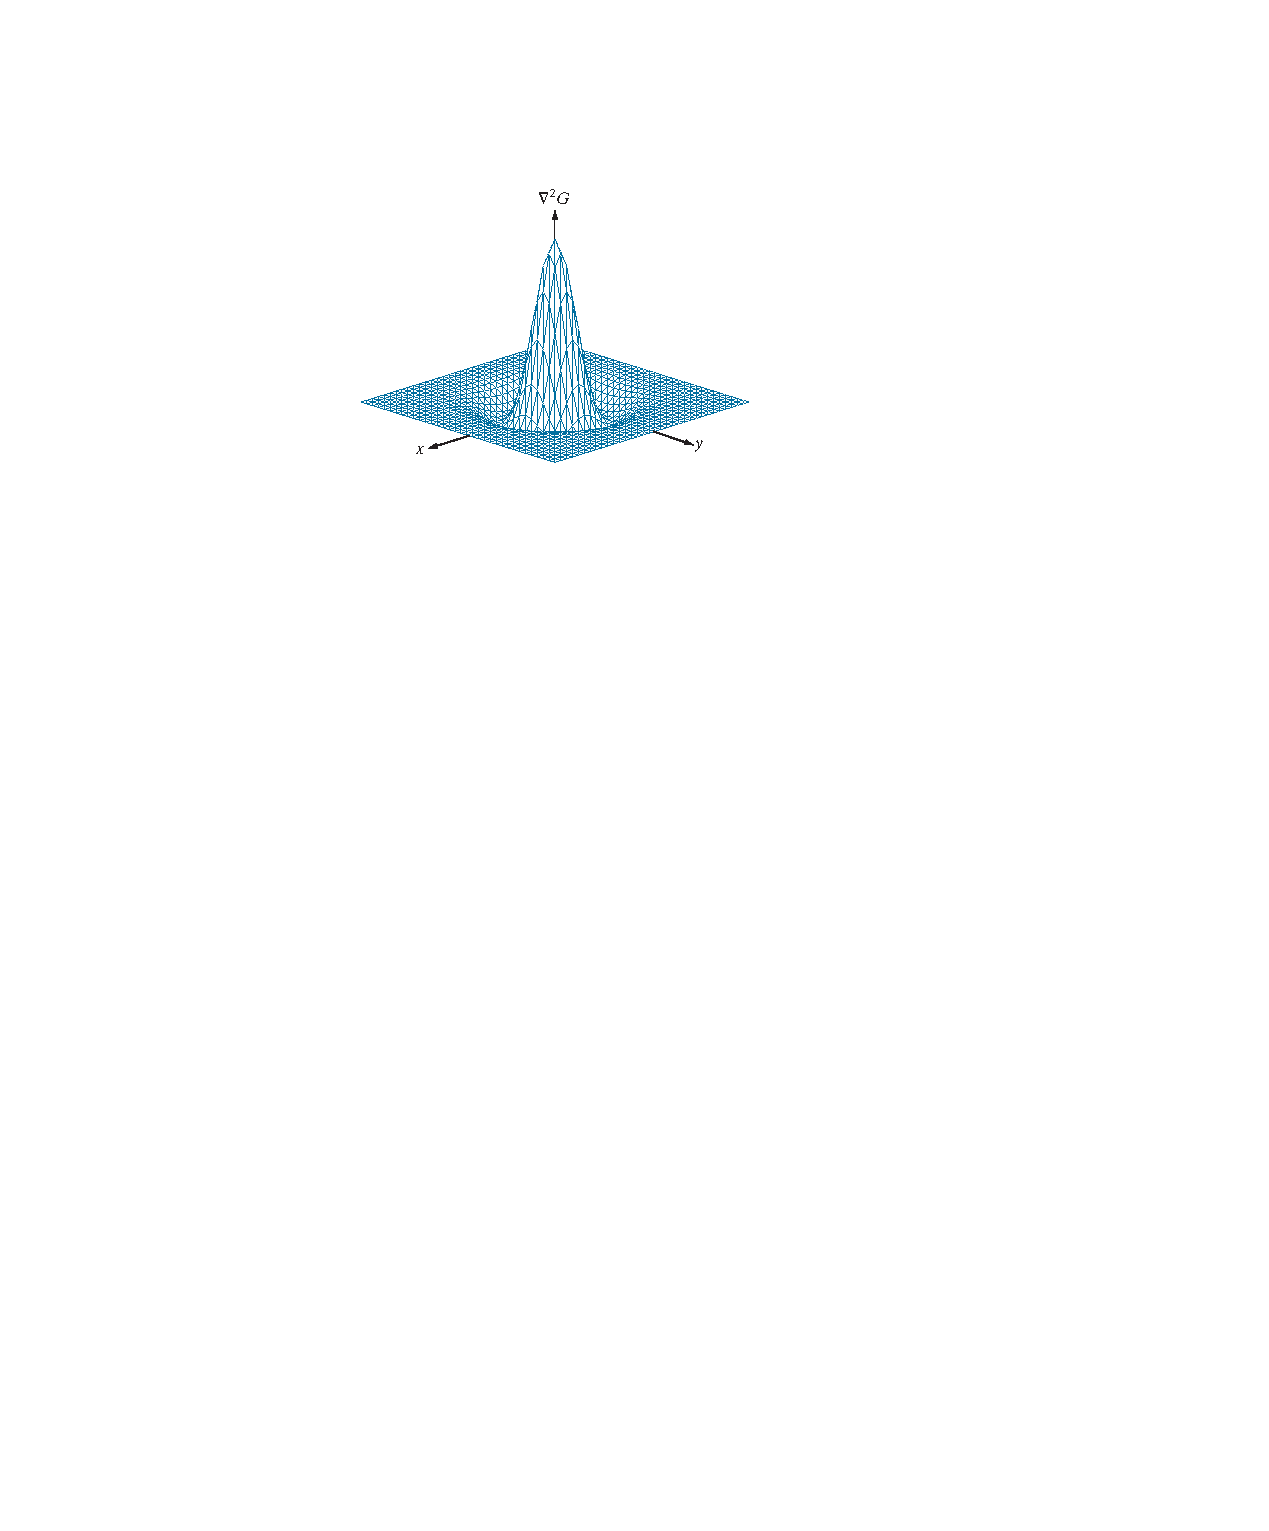
\includegraphics[width=\textwidth]{fig/LoG.pdf}
	\caption{3-D plot of the negative of the LoG.}
\end{marginfigure}

\begin{figure}[H]
	\centering
	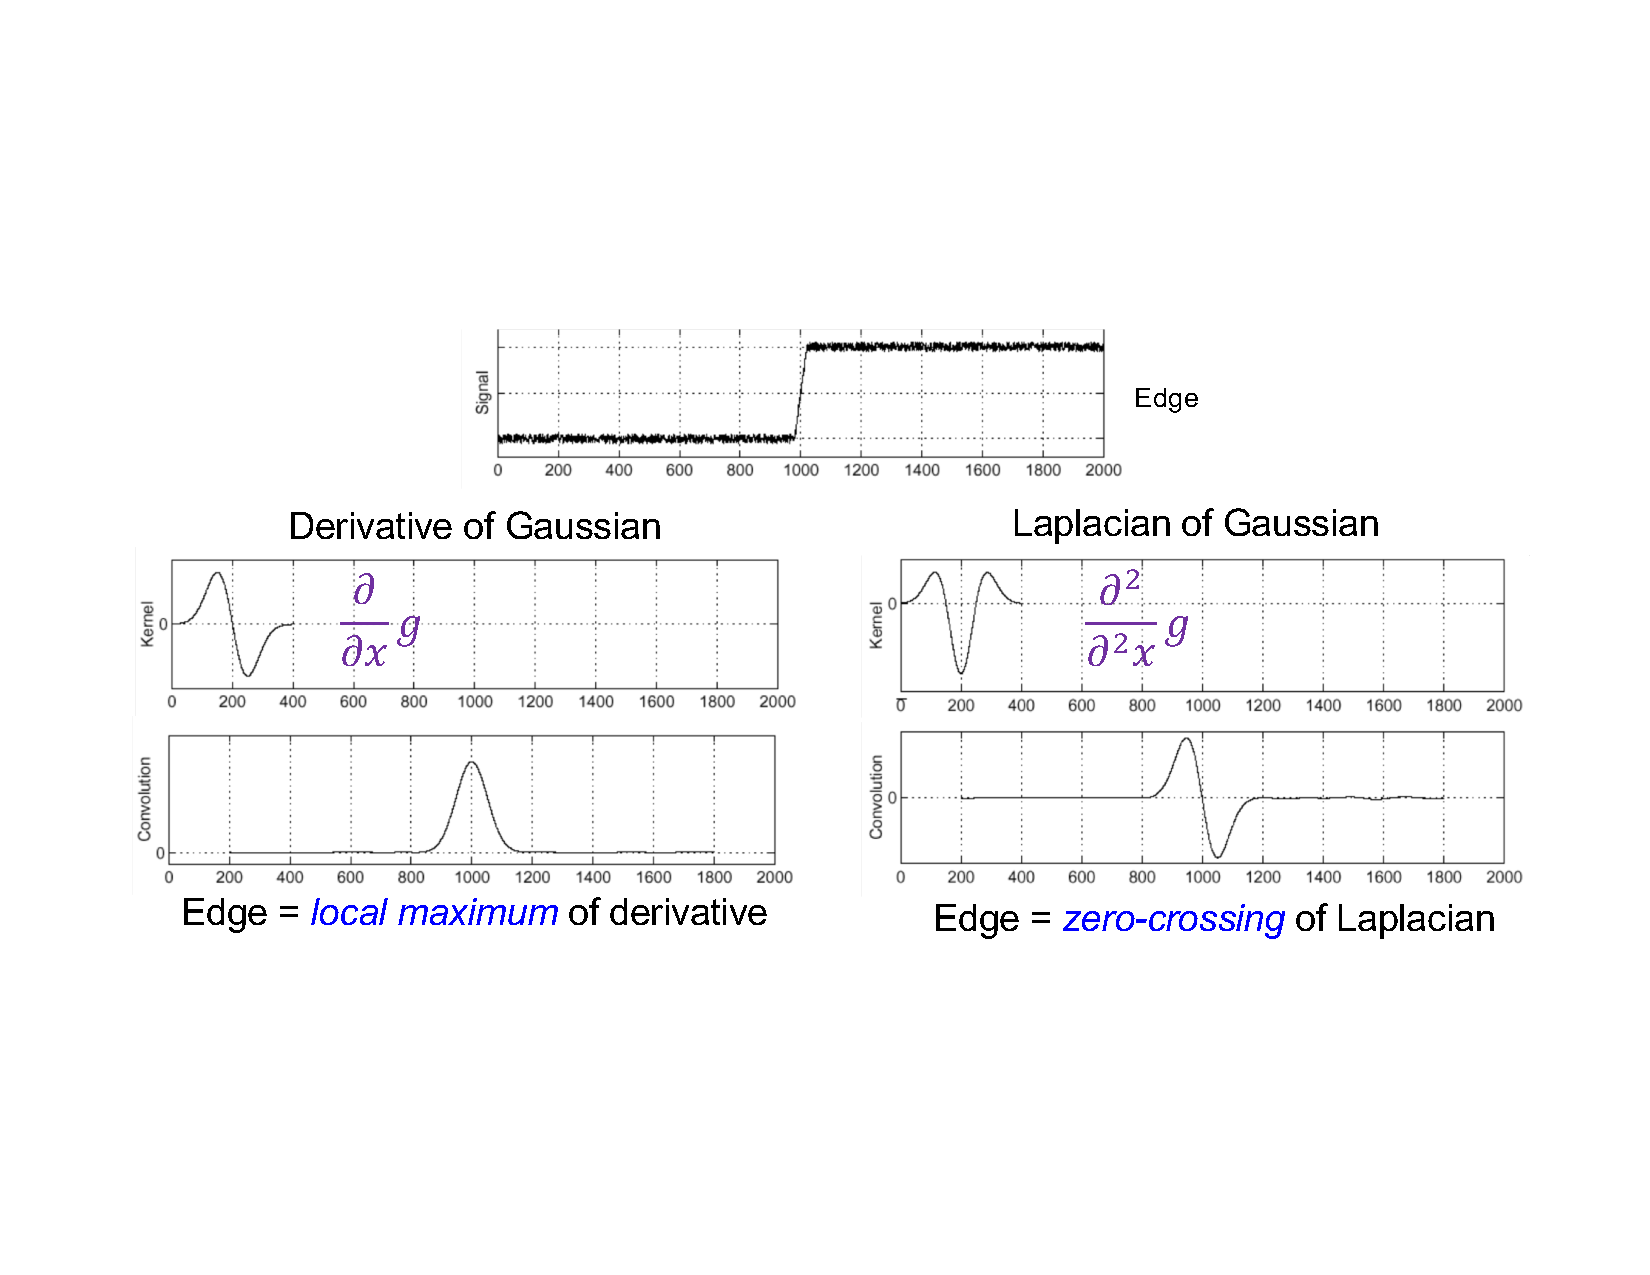
\includegraphics[width=.9\textwidth]{fig/Edge detection with LoG.pdf}
	\caption{\gspd 和\lpl 分别进行边缘检测\cite{marr1980theory}。}
\end{figure}

不仅如此,\lpl 相比于\gspd 还拥有一个更好的特性,即具有\emph{空间选择特性(Spatial Selection)}:% 插图
当\lpl 的尺度$\sigma$与信号的宽度匹配时,两者卷积会在原信号的中心位置有最大响应。

\begin{figure}[H]
	\centering
	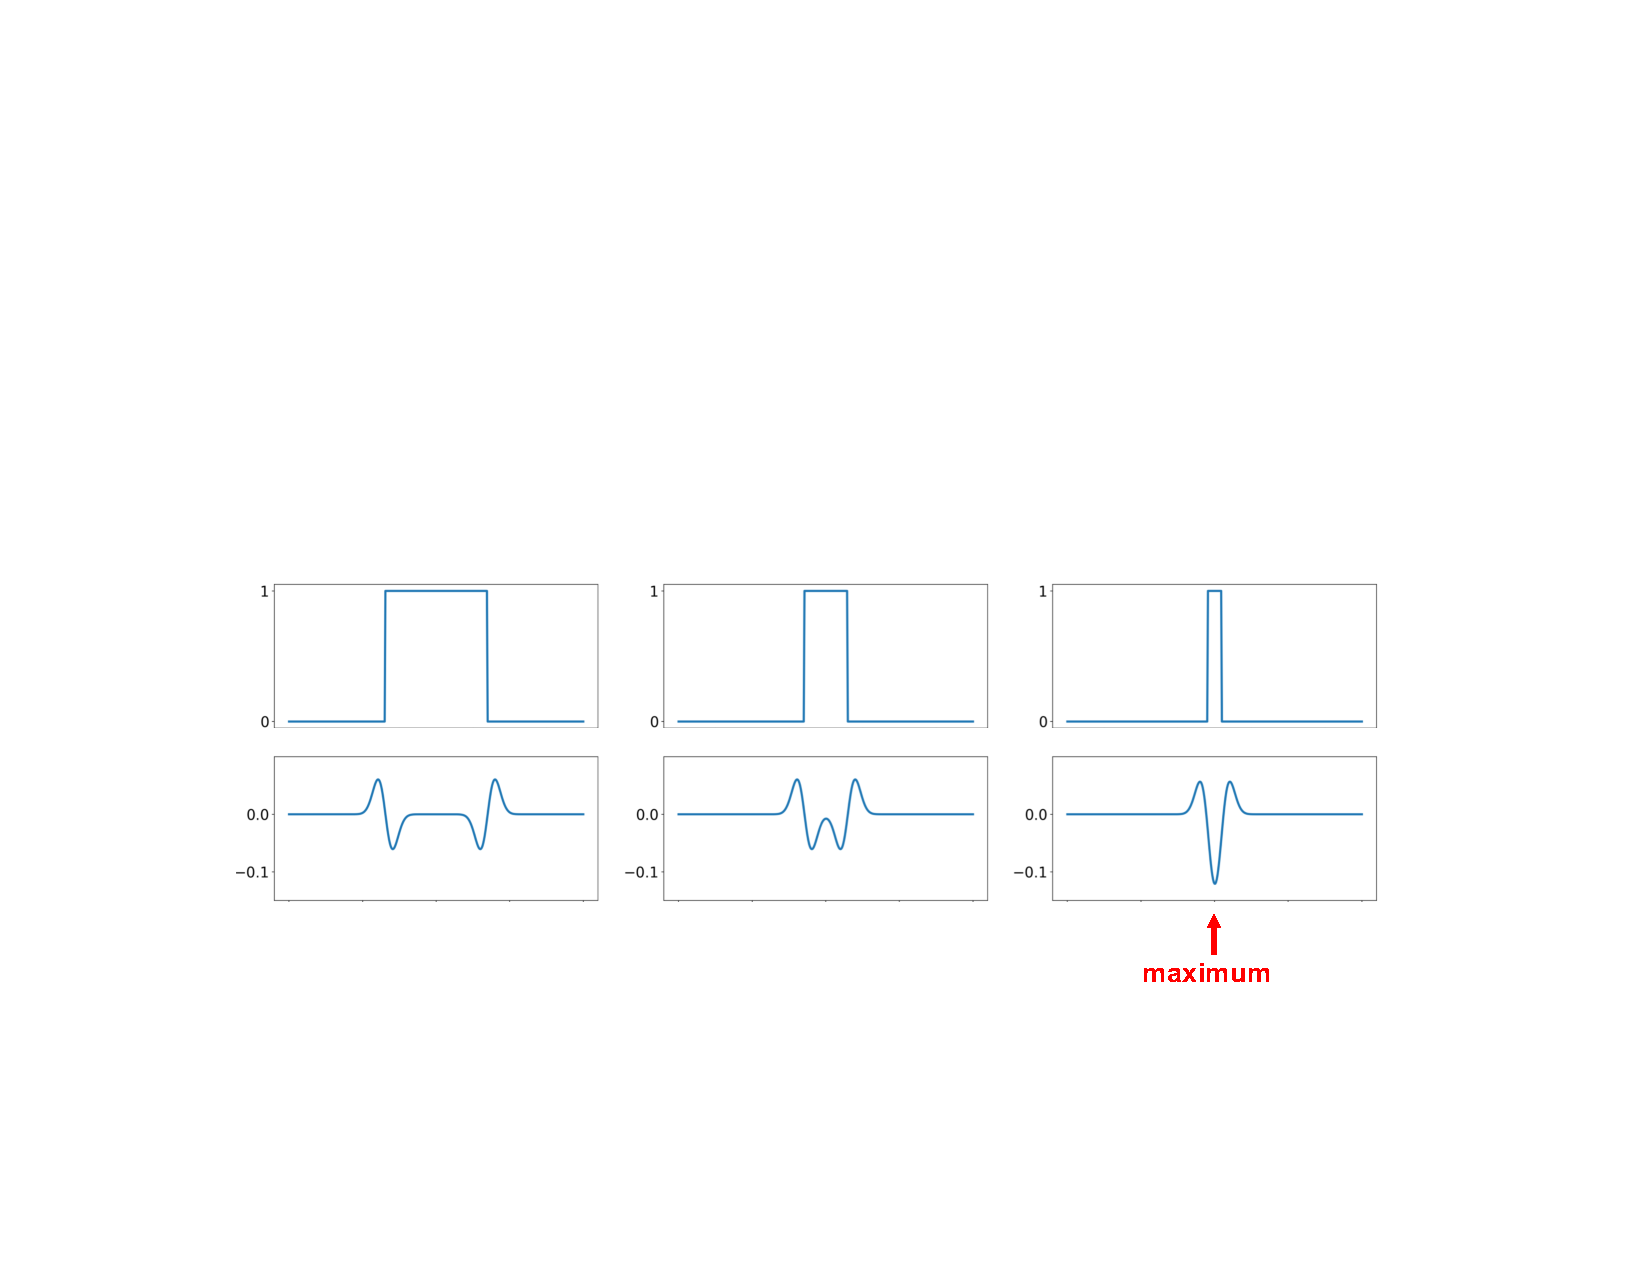
\includegraphics[width=.9\textwidth]{fig/spatial selection.pdf}
	\caption{\lpl 具有空间选择特性。}
\end{figure}

因此容易想到由\lpl 的空间选择特性,用一组尺度不一的\lpl 分别与某一尺度未知信号做卷积,通过判断响应值的大小最终确定该信号的尺度。而响应值最大时\lpl 与信号在尺度上到底存在什么数量关系呢?

\begin{marginfigure}
	\centering
	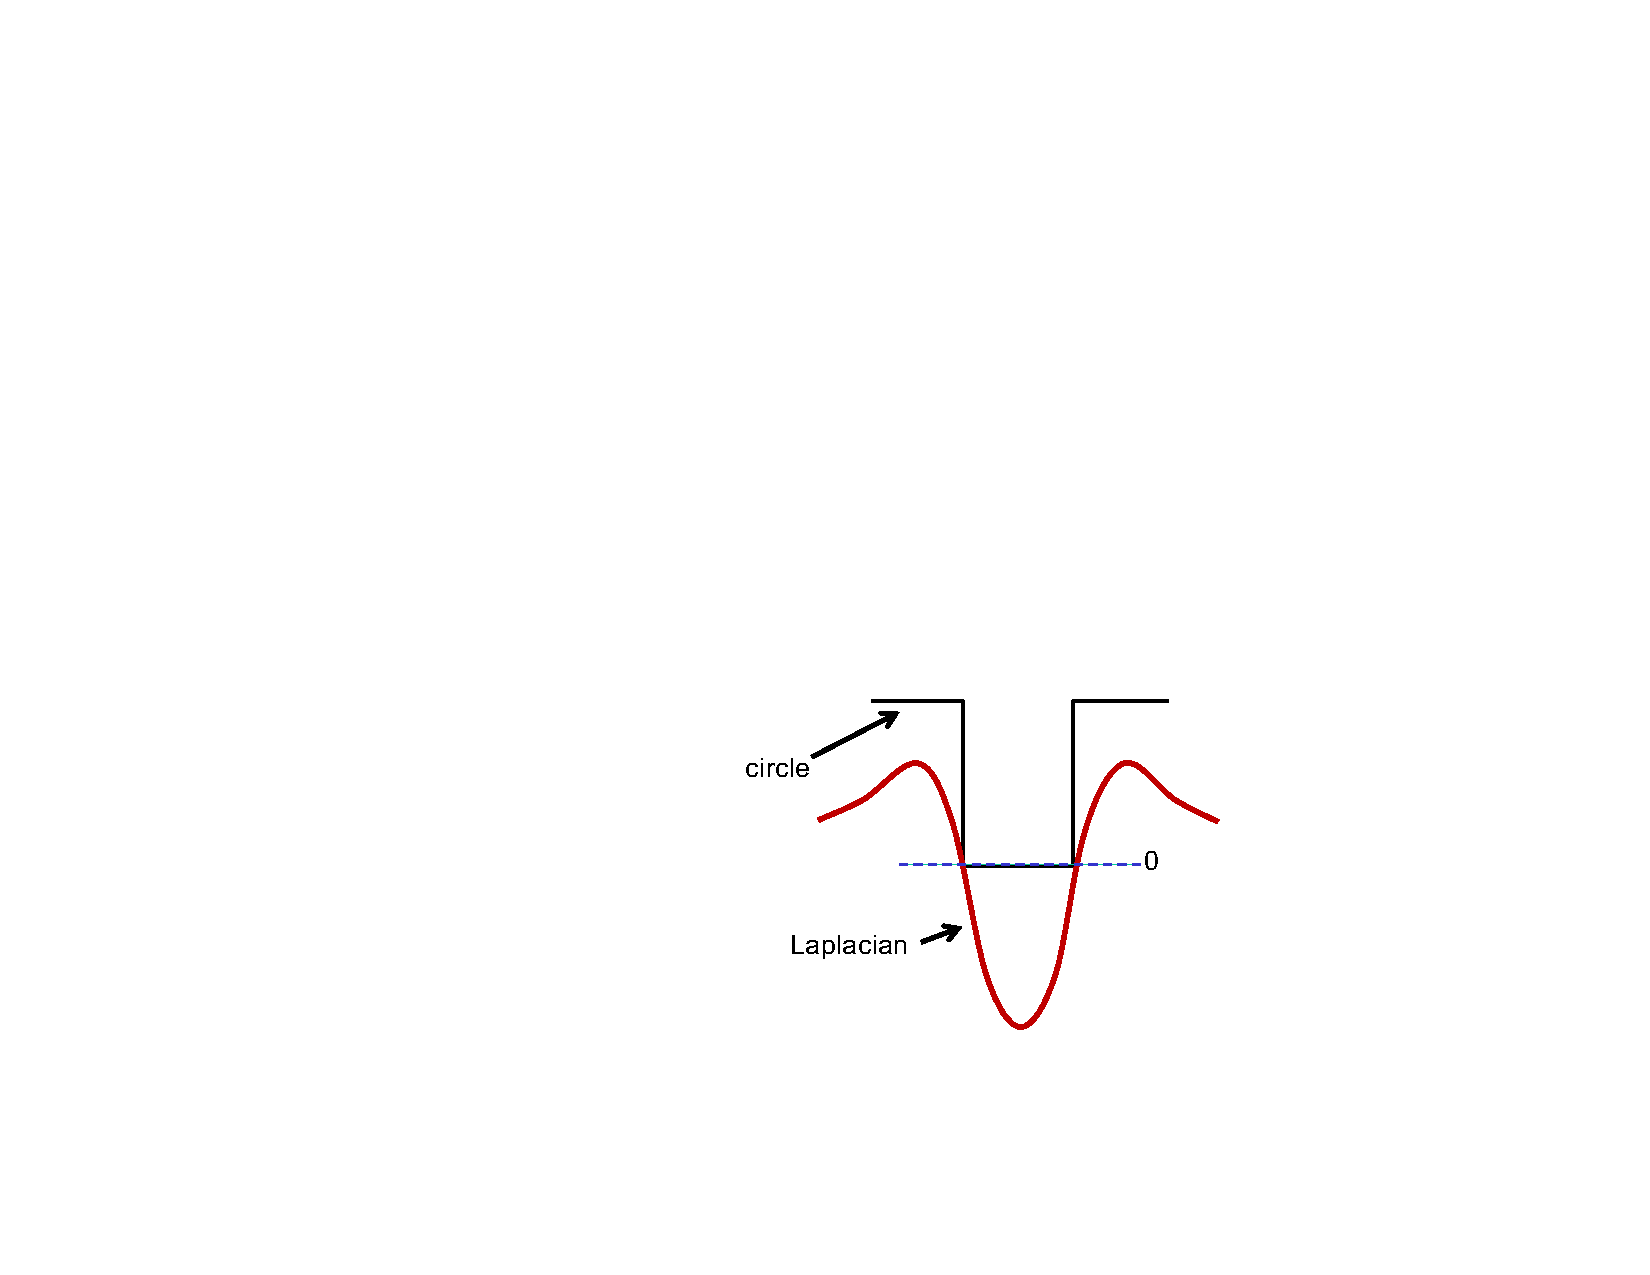
\includegraphics[width=\textwidth]{fig/LoG zero crossings-2.pdf}
	\caption{\lpl 的过零点刚好与信号卡住的情形。}
\end{marginfigure}

\begin{intu}
	当\lpl 的过零点刚好与信号卡住的时候,会在信号的中心点产生最大响应。于是,令
	\begin{equation*}
		\nabla^2_{\text{norm}}g = 0
	\end{equation*}
	得到$x^2+y^2=2\sigma^2$,即要想产生最大响应,信号的半径$r$应等于\lpl 过零点围成的半径$\sqrt{2}\sigma$。换句话说,与半径为$r$的信号产生最大响应的\lpl 参数$\sigma$应当满足:$\sigma=r / \sqrt{2}$。
	% TODO
	\begin{figure}[H]
		\centering
		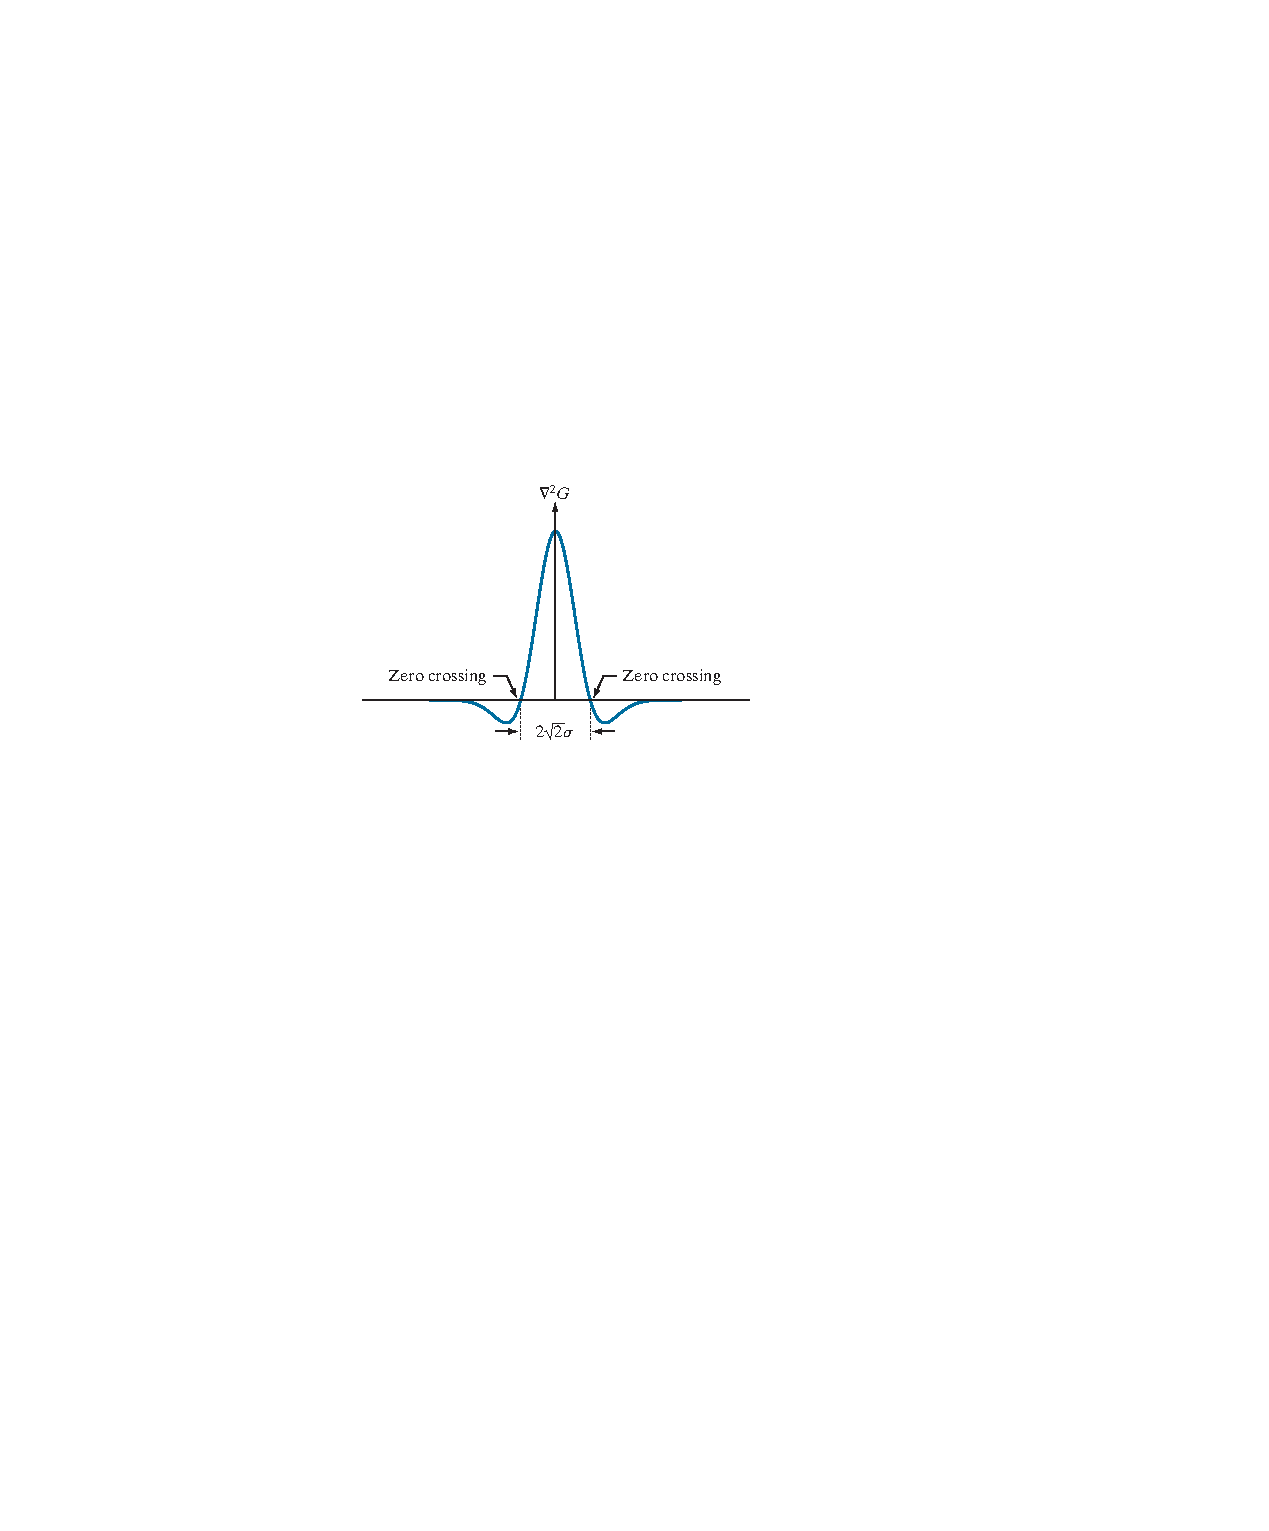
\includegraphics[height=6cm]{fig/LoG zero crossings.pdf}
		\caption{\lpl 过零点}
	\end{figure}
\end{intu}

直觉上看,信号的尺度和与之产生最大响应值的\lpl 的$\sigma$存在上述关系。但事实上,卷积的响应值会随着尺度$\sigma$的增大不断衰减,因此在此之前还必须对响应值进行\emph{尺度补偿(scale normalize)}:
\begin{equation}
	\nabla^2_{\text{normalized}}g=\eqnmarkbox[emph2]{compensate}{\sigma^2}\left(\frac{\partial^2 g}{\partial x^2} + \frac{\partial^2 g}{\partial y^2}\right)
\end{equation}

\section{图像尺度空间}

对于图像信号,如果希望找到图像上以某一点为中心所在局部特征的尺度$r$,就可以使用一组尺度($\sigma$)不同的归一化\lpl 分别对图像做卷积。\figref{fig:Scale-space blob detector}表示了一组用多尺度\lpl 相卷积得到的图像尺度空间,%
在纵向找到该位置处响应值最大时的\lpl,然后根据其参数$\sigma$即可计算局部特征的尺度$r = \sqrt{2}\sigma$。%
\begin{marginfigure}
	\centering
	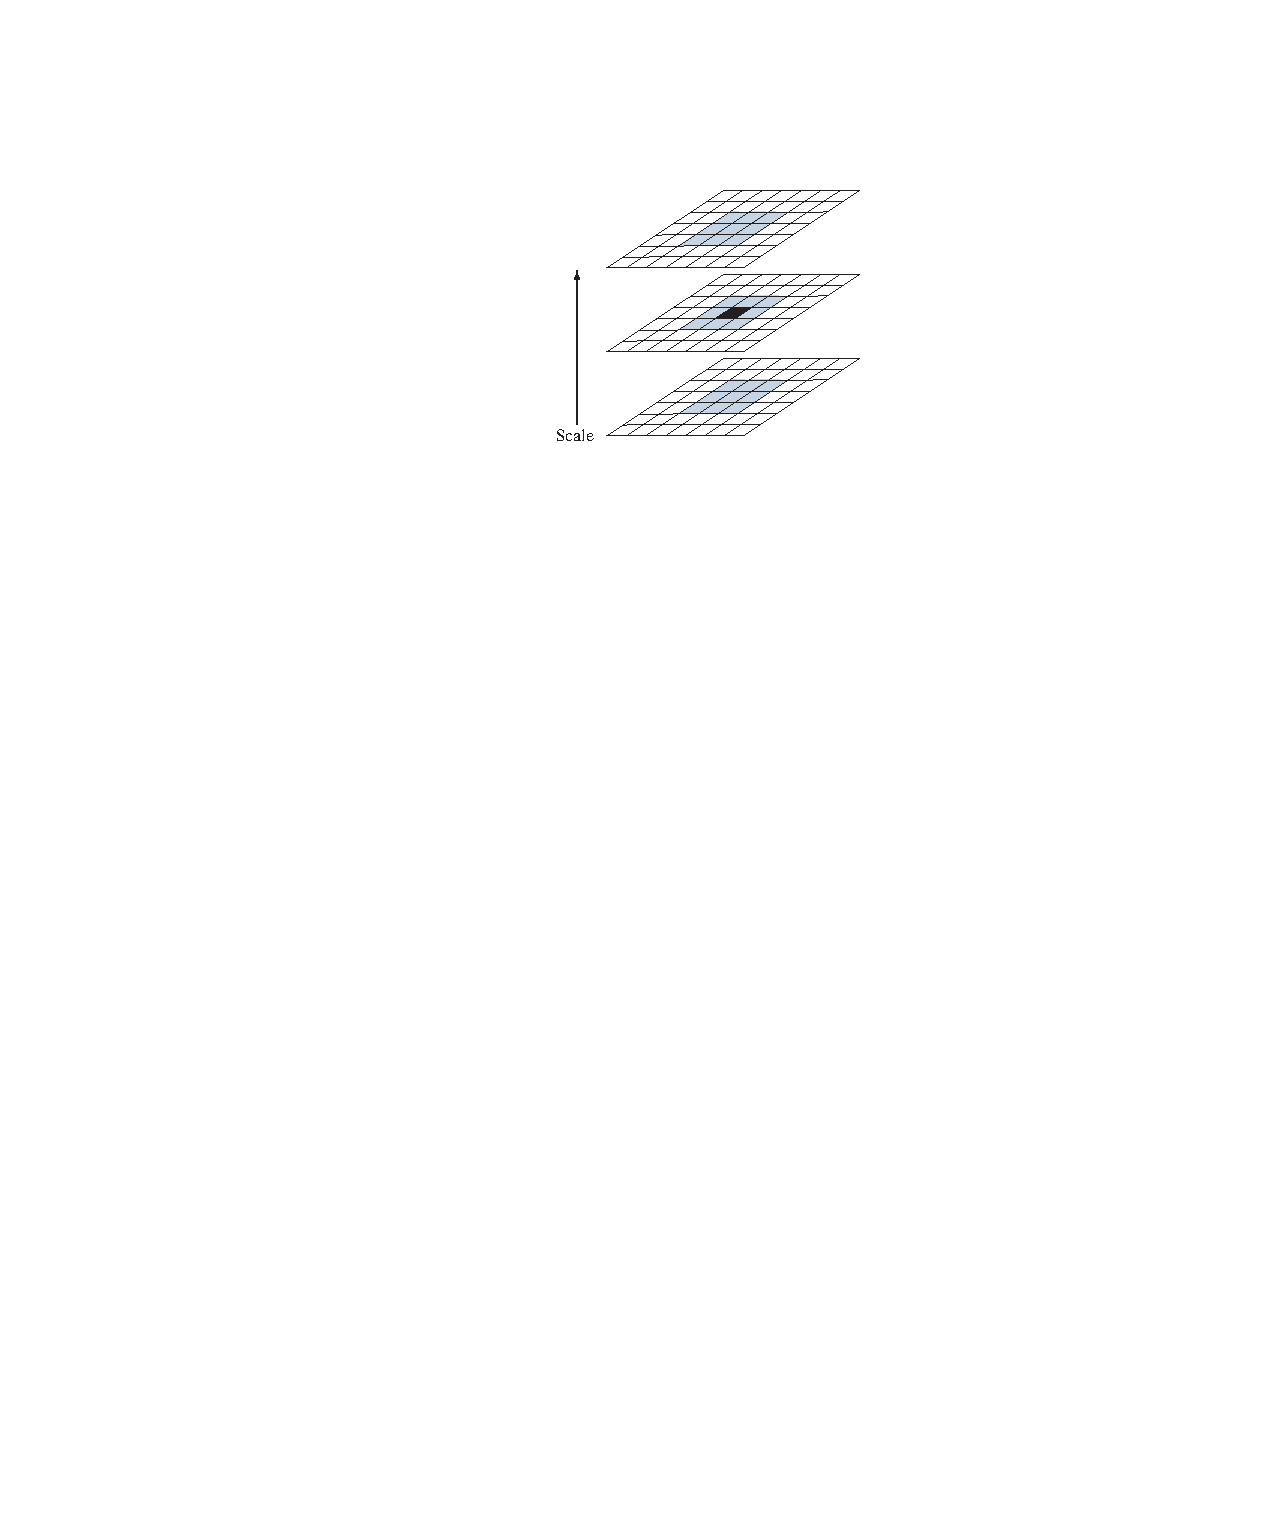
\includegraphics[width=\textwidth]{fig/Scale-space blob detector.pdf}
	\caption{图像尺度空间特征检测}
	\label{fig:Scale-space blob detector}
\end{marginfigure}


要对图像提取局部特征时,就对每一个像素坐标进行上面的操作。但是实际中并不会将\lpl 组的尺度划分得过细以逼近响应极值,这样将造成过大的计算消耗,同时意味着每一个像素坐标只能对应一个局部特征。因此,通常每三个\lpl 尺度进行比较,如果中间的响应值大于上下,则认为中间这个位置为响应极值,从而可确定出其所对应局部特征的尺寸。

然后横向在响应极值所在的尺度平面上看,周围像素其对应的响应也可能是极值,这也就导致了图像中局部特征可能会大量重叠。因此还需要进行\emph{非极大值抑制},其思路就是在确定响应极值时,不仅纵向跟自己位置进行比较,还需要跟图像尺度空间当中周围的26个像素相比,如果该响应值仍然最大,则保留这一处这一尺度的局部特征,否则遗弃该位置。

至此介绍了在图像尺度空间进行\emph{尺度搜索}和\emph{非极大值抑制}两个关键环节。但是上述过程仍然需要进行大量计算,为此\cite{mikolajczyk2001indexing}提出了Harris-Laplacian方法,先找出图像当中所有的Harris角点,然后只在这些点周围建立尺度空间,进行\lpl 的尺度分析。Harris对光照、平移、旋转具有不变性,再加上\lpl 的空间选择特性带来具有尺度不变性的局部特征。再到后来\cite{lowe2004distinctive}提出了更加高效的\sift 特征提取方法。

\part{Keypoint Detection}\label{part:Keypoint detection}

\part{SIFT Descriptor}\label{part:SIFT descriptor}

\part{Using SIFT for Image Matching}\label{part:Matching descriptors}

基于前面提取\sift 特征点、描述\sift 特征点的过程,本部分进一步介绍如何进行多视角图像间特征点的匹配,并展示一个最终的实验结果。

\section{描述子匹配}

寻找一幅图像中某个特征点在另一幅图像中的对应,即寻找与之描述子最为接近的特征点。衡量两个描述子(即特征向量)之间距离的方式有很多,例如欧氏距离(2-范数),汉明距离等。这里,我直接使用欧氏距离,并且以暴力匹配的方式寻找描述子之间的匹配关系。

同时,不一定一幅图像中的每一个描述子都能在另一幅图像中找到对应点,因此可以对描述子之间的距离设置一个上限;并且可以每次选取距离最近的两个描述子,如果最接近的描述子距离上要明显小于次接近的描述子,则可认为最接近的描述子是可靠的。

\section{实验效果:图像特征匹配}

\part{Summary}\label{part:Summary}

\sift 是一种在计算机视觉领域中传统而又常用的图像处理算法。SIFT算法的主要意义在于其能够有效地提取图像中的特征,并通过特征匹配来实现图像的识别、匹配、定位等应用。最后再总结一下其最为基本的五大步骤:
\begin{enumerate}
    \item \textbf{构建尺度空间} \quad \lpl 所具有的空间选择特性为特征的尺度分析提供了方法。\sift 当中用高斯差分近似\lpl 以高效构建尺度空间(\equref{equ: DoG and LoG})。其具体过程首先构建了高斯金字塔,然后在每个尺度上,通过相邻两个高斯模糊后的图像相减,得到差分图像。将每个尺度的差分金字塔中相同位置的差分图像组合成一个3D张量,构成尺度空间。每个张量代表了在一个特定尺度下图像的局部特征。在构建尺度空间的过程中,\octave 的层数$o$,每层\octave 包含的尺度个数$S$,以及高斯差分函数的$\sigma$参数是三个重要的经验参数,它们决定了所能检测到的尺度范围,以及每个尺度之间的差异程度。为了保证图像的尺度不变性,它们的值需要根据特征尺度进行自适应调整,以便提取到不同尺度下的关键点。
    \item \textbf{定位关键点} \quad 定位关键点的过程就是进行非极大值抑制的过程,即既要保证特征在某个高斯差分上的响应超过阈值,还要保证其在 \DoG 尺度空间比它的领域都要大。首先,对每个尺度的差分金字塔中的每个像素,如果其响应值超过了阈值,则继续检查其周围3x3x3邻域内的26个像素,确定其是否为该邻域的极值点。对于每个尺度的差分金字塔,将极值点的坐标和所处的尺度记录下来,形成关键点集合。
    \item \textbf{主方向分配} \quad 分析以关键点为中心的局部图像块的梯度主方向。图像的梯度分析对光照变化更为鲁棒,而梯度主方向的确定可以消除特征的旋转不确定性。按\equref{equ: compute gradient}方式计算以每个\sift 特征关键点为中心提取出$16\times 16$的局部图像块的梯度。接下来通过构建梯度方向直方图的方式确定主方向。在找到这个主方向之后,通过对关键点周围的图像区域进行旋转的方式, 将该主方向变换到统一的标准方向。
    \item \textbf{特征描述} \quad 每个关键点生成一个具有区分度和鲁棒性的特征描述符,用于表示关键点周围的图像信息。首先将关键点所在的尺度空间的图像分为$4\times 4 =16$个大小相等的子区域,为每个子区域构建长度为$8$的梯度方向直方图。将这$16$个梯度方向直方图拼接在一起后进行归一化,得到最终的$128$维特征向量。
    \item \textbf{描述子匹配} \quad 通过比较两张图像的特征描述符,找出相似的特征点,实现图像间的匹配和识别。可直接使用欧氏距离,并且以暴力匹配的方式寻找描述子之间的匹配关系。
\end{enumerate}

实验结果表明,所实现的\sift 算法的特征匹配正确率$77.8\%$,能够较为鲁棒地解决尺度、旋转等变化条件下的特征匹配任务。另外,实验中出现的两对错误匹配也表明,仅仅依靠局部特征描述无法区分重复的纹理特征。

可以看出,\sift 特征提取与匹配算法有着清晰而又复杂的处理流程,并且依靠许多经验参数,但这还只是最为基础的一种实现方式。将来在此基础还可以做出如下改进:
\begin{itemize}
    \item \textbf{关键点的精确定位}\quad 在离散采样中搜索到的极值点不一定是真实空间的极值点,因此对尺度空间DoG函数进行泰勒展开,在近似连续域上计算其极值点,从而实现关键点的精确定位。
    \item \textbf{增加关键点对视角的鲁棒性}\quad 对视角变化具有一定的鲁棒性,但是在大视角变化下其性能会受到影响。由于透视变换的作用,在数据库图像上原本接近圆形的特征会在查询图像上畸变为椭圆,从而导致无法匹配。\cite{mikolajczyk2004scale}中提出了基于二阶协方差矩阵的仿射不变特征点检测算法。
    \item \textbf{去除边缘上的点}\quad 由于DoG对图像中的边缘有比较强的响应值,而一旦特征点落在图像的边缘上,这些点就是不稳定的点。它们很难定位,具有定位歧义性,且容易受到噪声的干扰而变得不稳定。根据主曲率比值来判断关键点是否为稳定的特征点,如果不稳定则删除。
\end{itemize}


% --------------------->>参考文献<<-----------------------
\bibliography{egbib}
\end{document}
